\section{Introduction}

Key-Value stores are used in many important websites. For example, Dynamo is
used at Amazon~\cite{dynamo}; Redis is used at Github, Digg, and Blizzard
Interactive~\cite{Reddi10}; and Memcached is used at Facebook, LinkedIn and
Twitter~\cite{memcached, Petrovic08}. These applications store Key-Value pairs
and commonly function as a cache for frequently recurring computations, such as
complex SQL queries. Therefore, tuning the performance of these storage systems
is essential for building efficient large-scale web services. Because latency
is critical for these applications, many optimizations have been explored that
aim to reduce the response latency of these systems. 

\begin{figure}[b]
\begin{center}
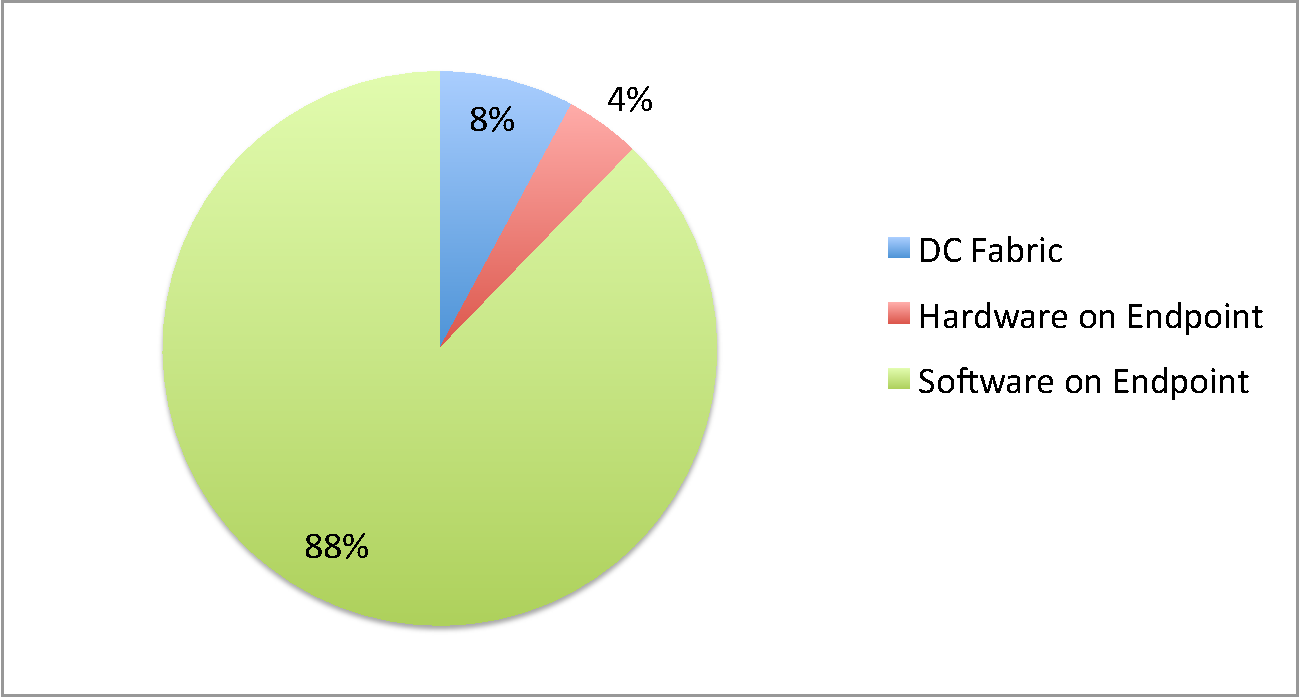
\includegraphics[width=\linewidth]{softwarelag.pdf}
\caption{Components of memcached request latency in a datacenter}
\label{fig:lag}
\end{center}
\end{figure}

When analyzing the performance of large kv stores, we see that there are many
different sources of latency in a GET request, but not all contributions are
equal. One study of a typical datacenter application, summarized in
Figure~\ref{fig:lag}, indicates that software at the endpoint accounts for
$88\%$ of the total request latency~\cite{Kapoor2012}. Thus, if we can improve
the latency of a single node, we can make substantial improvements to the
total request latency in a memcached cluster. This is the focus of this paper.

We propose incorporating a dedicated cache on each node whose sole job is to
serve memcached GET requests. This approach is effective due to the high skew
that is present in the distribution of keys in realistic workloads, where a
small number of keys make up most of the requests seen at a single node. GET
requests are simple enough to handle with specialized hardware, allowing us to
bypass the software networking stack entirely. Our preliminary evaluation shows
that we reduce latency by a factor of ten for keys served from the accelerator
when compared with a software implementation on the same board.
